\documentclass[a4paper,10pt]{article}

%A Few Useful Packages
\usepackage{marvosym}
\usepackage{fontspec} %for loading fonts
\usepackage{multirow}
\usepackage{amssymb} 
\usepackage{xcolor,lipsum}
\usepackage{titlesec}

\usepackage{xunicode,xltxtra,url,parskip} 	%other packages for formatting
\usepackage{array}
\RequirePackage{color,graphicx}
\usepackage[usenames,dvipsnames]{xcolor}
\usepackage[big]{layaureo}
\usepackage{tabu}%better formatting of the A4 page
% an alternative to Layaureo can be ** \usepackage{fullpage} **
\usepackage{supertabular} 				%for Grades
\usepackage{titlesec}					%custom \section
   					%custom \section


\usepackage{geometry}
 \geometry{
 a4paper,
 total={170mm,257mm},
 left=15mm,
 right = 20mm,
 top = 10mm, 
 tmargin = 10mm,
 bottom = 5mm,
 bmargin = 5mm,

 }









%Setup hyperref package, and colours for links
\usepackage{hyperref}
\definecolor{linkcolour}{rgb}{0,0.2,0.6}

\hypersetup{colorlinks,breaklinks,urlcolor=linkcolour, linkcolor=linkcolour}

%FONTS
\defaultfontfeatures{Mapping=tex-text}
%\setmainfont[SmallCapsFont = Fontin SmallCaps]{Fontin}
%%% modified for Karol Kozioł for ShareLaTeX use
\setmainfont[
SmallCapsFont = Fontin-SmallCaps.otf,
BoldFont = Fontin-Bold.otf,
ItalicFont = Fontin-Italic.otf
]
{Fontin.otf}
%%%

%CV Sections inspired by: 
%http://stefano.italians.nl/archives/26
\titleformat{\section}{\Large\scshape\raggedright}{}{0em}{}[\titlerule]
\titlespacing{\section}{0pt}{3pt}{3pt}
%Tweak a bit the top margin
%\addtolength{\voffset}{-1.3cm}

%Italian hyphenation for the word: ''corporations''
\hyphenation{im-pre-se}

%-------------WATERMARK TEST [**not part of a CV**]---------------
\usepackage[absolute]{textpos}
\usepackage{placeins}

\setlength{\TPHorizModule}{20mm}
\setlength{\TPVertModule}{\TPHorizModule}
\textblockorigin{2mm}{0.65\paperheight}
\setlength{\parindent}{0pt}



%----------------BREADCRUMBS FOR TECHNICAL SKILLS



\definecolor{mybreadcolor}{rgb}{0.87,0.63,0.87}









%--------------------BEGIN DOCUMENT----------------------
\begin{document}



\pagestyle{empty} % non-numbered pages

\font\fb=''[cmr10]'' %for use with \LaTeX command

%--------------------TITLE-------------
\par{\centering
		{\Huge  \textsc{Resume}
	}\bigskip\par}





%--------------------SECTIONS-----------------------------------
%Section: Personal Data

\titleformat{name=\section}[block]
  {\sffamily\large}
  {}
  {0pt}
  {\colorsection}
\titlespacing.*{\section}{0pt}{\baselineskip}{\baselineskip}

\newcommand{\colorsection}[1]{%
  \colorbox{blue!25,}
  {\parbox{\dimexpr\textwidth-20\fboxsep}{\thesection\ #1}}
  }



\par	


{\Large  \textbf{Viplav. P .PATIL }}

{\large 
\par
M.Tech Student with Excellent  Problem Solving 
 Skills and ability to \par perform well in a  team.Passionate about Coding.
}

%{\large  Software Developer }

 \vspace{1mm}


\par	
{\large \textbf{National Institute of Technology(NIT),Durgapur.} 
 }
 
 \par
{\large \textbf{Computer Science,} 
 }
 
 
\par	

\includegraphics[width=0.03\textwidth,left]{gmail} \quad {\large  Viplavdhande91@gmail.com}

\par

\includegraphics[width=0.03\textwidth,left]{linkedin}
\quad{\large  https://www.linkedin.com/in/viplav-patil-a5789028/}

\par

\includegraphics[width=0.03\textwidth,left]{mobile}
\quad{\large  +91-9421679707}
\par

\includegraphics[width=0.03\textwidth,left]{GitHub-Mark}
\quad{\large   https://github.com/viplavdhande91}
\par	

\vspace{-58mm}

    \begin{figure}[h]
\raggedleft

    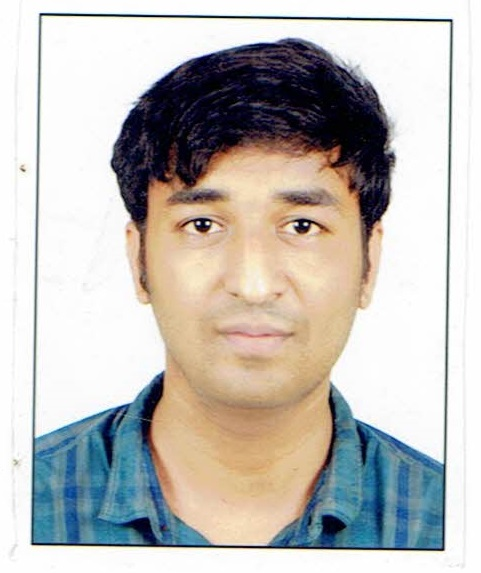
\includegraphics[width=0.25\textwidth,right]{CCI09172017}    \end{figure}
    \FloatBarrier






\section{M.Tech Academic SGPA:}

\begin{tabu} to 0.8\textwidth { | X[0.7] | X[3] |  }
 \hline
 
 \Large
 SEMISTER  & \Large
  Semister Grade Average Point (On 10 Scale)   \\
\hline
\large Semister IV & 10.0   \\  
\hline
\large Semister III & 9.0   \\
 \hline
 \large Semister II & 7.75  \\
 \hline
\large Semister I & 6  \\
 \hline
\end{tabu}



\vspace{1mm}


\section{Academic Details:}

\begin{center}
\begin{tabular}{ | m{2.0cm} | m{7.0cm}| m{3.5cm} | m{3cm} | } 
\hline
\textbf{Degree} & \textbf{Institute}    & \textbf{Year of Passing}  & \textbf{Percentage/CGPA }  \\ 
\hline
M.Tech (CSE)  & National Institute of Technology\newline\textbf{\small (NIT,Durgapur)}   & June,2021 & CGPA 7.83/10\\


\hline
B.E\newline(Computer Engineering) & SSBT’s COET,Bambhori

\textbf{\small (Affiliated to North Mahrashtra University,Jalgaon)}& July 2017  & CGPA 6.69/10 \\

\hline
HSC  & N.H.Ranka Jr.College,Bodwad\newline
{\small (Maharashtra State Board)}& June 2010 & 71.33 \% \\

\hline
SSC & N.H.Ranka HighSchool ,Bodwad\newline
{\small (Maharashtra State Board)}
  & May 2007 & 62.46 \%\\ 
\hline
\end{tabular}
\end{center}








\iffalse
\section{B.E Academic SGPA:}

\begin{tabu} to 0.8\textwidth { | X[l] | X[l] |  }
 \hline
 
 \Large
 SEMISTER  & \Large
  Semister Grade Average Points(On 10 Scale)   \\
\hline
\large Semister I & 5.61   \\
 \hline
 
\large Semister II & 6.78  \\
 \hline
 
 \large Semister III  &  5.52 \\
 \hline
 
\large  Semister IV & 6.83  \\
 \hline
 
\large Semister  V &   6.78 \\
 \hline
 
\large Semister VI &   7.57\\
 \hline
 
\large Semister VII  & 7.22  \\
 \hline
 
 \large Semister VIII & 7.22  \\
 \hline

\end{tabu}

\fi

\vspace{1mm}





\section{TECHNICAL Skills:}

\begin{tabu} to 1.1\textwidth { | X[0.15] | X[2] |  }
 %\large  Area of Interest:  & Computer Networks,Data Structures,Database Managment Systems\\
 \hline

\hline



\large  Skills :  & 
\colorbox{mybreadcolor}{C}{}
\enspace\colorbox{mybreadcolor}{Python}{} 
\enspace\colorbox{mybreadcolor}{Java}{}
\enspace\colorbox{mybreadcolor}{Data Structures \& Algorithms}{}
\enspace\colorbox{mybreadcolor}{Deep Learning}{}
\enspace\colorbox{mybreadcolor}{LINUX}{}
\enspace\colorbox{mybreadcolor}{SQL }{}
\enspace\colorbox{mybreadcolor}{Django}{}

%\bigbreak
\vskip 0.05in


\colorbox{mybreadcolor}{Problem Solving}{}
\enspace\colorbox{mybreadcolor}{Operating Systems}{}
\enspace\colorbox{mybreadcolor}{Computer Networking}{}
\enspace\colorbox{mybreadcolor}{Git \& Github}{}
\\


\hline
\end{tabu}






\section{PROJECTS:}

\renewcommand{\labelitemi}{$\blacksquare$}
 %\renewcommand\labelitemii{$\square$}


 
 
 
\vspace{1mm}

 
 
 \begin{itemize}
   \item {\large PERSON PREDICTION USING DEEP-LEARNING(CNN)}
   
 \end{itemize}


\begin{tabu} to 1.1\textwidth { | X[0.4] | X[3] | }

 
 \hline

\large Description & AUTOMATED SYSTEM
TO DETECT PERSON ENTERING AN ORGANIZATION PREMISES USING CONVOLUTIONAL NEURAL
NETWORKS(DEEP LEARNING).  \\
 
 
\hline

 
\end{tabu}
 
 
 
 
 
  
 
 \begin{itemize}
   \item {\large {EFFICIENT INCOME TAX
MANAGEMENT WEB PORTAL}}
   
 \end{itemize}


\begin{tabu} to 1.1\textwidth { | X[0.4] | X[3] | }

 \hline
\large  Description & Income Tax Form Filling  and Uploading Necessary Tax Documents on Web Portal designed for Employees.This Project is Developed for NIT Durgapur Tax Payer Employees.    \\
 

 

\large     & 

 \textbf{\small(Current Stage : Production)\newline
 \textbf{\small PRODUCTION URL: }https://taxapp87.herokuapp.com/}

\\
\hline

 
\end{tabu}
 
 
 
 
 
 
 
 
 
 
 
 
 \begin{itemize}

   \item {\large {EFFICIENT \& OPTIMIZED E-COMMERCE SHOPPING(KICKS).}}
   
 \end{itemize}


\begin{tabu} to 1.1\textwidth { | X[0.4] | X[3] | }

 \hline
\large  Description & Functional and Optimized E-commerce B2C Website developed using Django Framework at Backend for Coloured-Sneakers Selling with complete Online Payment Gateway(Paytm) Integration. 
\newline
 \textbf{\small(Current Stage : Production)}\newline
  \textbf{\small PRODUCTION URL: } http://kicks92.herokuapp.com/


\newline https://github.com/viplavdhande91/kicks 

\\
 

 \hline

 
\end{tabu}
 
 
 

 
 
 
 
 
 
 
 
 
 
 
 
 

 %\begin{itemize}

  % \item {\large{Optimized Web Portal for Employer}}
   
% \end{itemize}


%\begin{tabu} to 1.1\textwidth { | X[0.5] | X[3] | }

% \hline
%\large  Description & This Implementation facilitates on %Attendance Management,Employees Salary Management,Advance %Amount taken Management with Integration of Personal secured %dashboard for owner.    \\
 

 
 

%\large    & \textbf{\small(Current Stage : Complete)\newline %http://nehabondesite.herokuapp.com/
%\newline https://.com/viplavdhande91/Resort-Management-system%.git }


%\\
%\hline

 
%\end{tabu}
 
 
 
 
 
 
 
 
 
 
 
 
 
% \begin{itemize}
%   \item {\large {A Dynamic Multi agent System Graph %Generation.
%}}
   
% \end{itemize}


%\begin{tabu} to 1.1\textwidth { | X[0.5] | X[3] | }

% \hline
%\large  Description & Generation of Multi Agent System %Architecture Dynamic Graph (MASAG) for Student Enrollement System.    \\
 

%\large    & \textbf{\small(Current Status : Completed)
%\newline https://.com/viplavdhande91/Multi-Agent-System-Graph%.git }


\\
%\hline

 
%\end{tabu}
 
 
 
 


 
 \vspace{1mm}

 
 
%
%\section{PUBLICATONS:}
%\begin{enumerate}
  % \item Paper Publication (Level: International Journal) 
  % \begin{itemize}
   % \item Viplav Patil,Vinaya Patil, Shiwani Suryawanshi, %Mayur Saner, Bhushan Sarode STUDENT PERFORMANCE %PREDICTION USING CLASSIFICATION DATA MINING TECHNIQUES %(IJSDR  ), Vol.2,Issue 6, June 2017, Paperid - %IJSDR1706021,Print ISSN: 2455-2631.
 
   %  \end{itemize}
    

%\end{enumerate}

%\vspace{1mm}
%\large 
%\par
%I hereby certify that the information specified above is %true,complete and correct to the best of my knowledge and %belief.  

\vspace{1mm}
         
%\begin{flushright}
%{\large Date : \today }
%\end{flushright}
%\par
%{\large Place : Durgapur(West Bengal) }

%\begin{flushright}
%{\LARGE Viplav .P. Patil}



 %   \begin{figure}[h]
%\raggedleft
   % 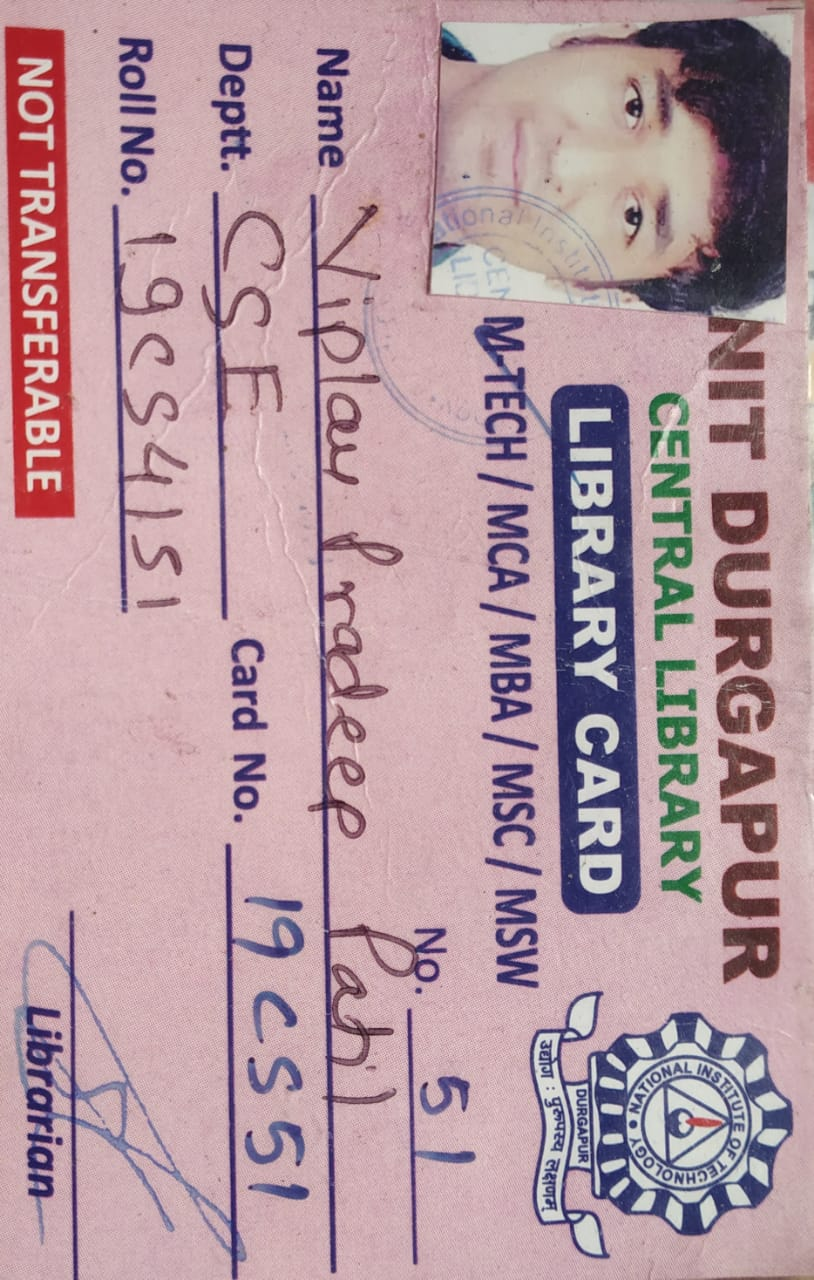
\includegraphics[width=0.25\textwidth,width=5cm, %height=6cm,right,angle=90]{libcard.jpeg}    \end{figure}
%\end{flushright}
   
%\newpage
%\par{\centering\Large \hypertarget{grds}{Master of 
%\bigskip


\end{document}
